\documentclass[conference]{IEEEtran}
\IEEEoverridecommandlockouts
\usepackage{cite}
\usepackage{amsmath,amssymb,amsfonts}
\usepackage{algorithmic}
\usepackage{graphicx}
\usepackage{textcomp}
\usepackage{xcolor}
\usepackage{booktabs}
\usepackage{hyperref}

\hypersetup{
    colorlinks=true,
    linkcolor=blue,
    filecolor=magenta,      
    urlcolor=cyan,
}

\begin{document}

\title{Foundations of Neural Networks: Perceptron, Adaline, Multi-Layer Perceptrons, and Bottleneck Representation Learning\\
\large Coursework Technical Report -- Neural Networks and Deep Learning (Spring 2025)}

\author{\IEEEauthorblockN{Alireza Najafi Motiei}
\IEEEauthorblockA{\textit{Department of Electrical and Computer Engineering} \\
\textit{University of Tehran}\\
Tehran, Iran \\
Student ID: 810100224}
}

\maketitle

\begin{abstract}
This report details the theoretical formulation, algorithmic implementation, and empirical evaluation of foundational artificial neural network architectures. We investigate: (1) Rosenblatt's Perceptron and its finite-step convergence guarantees on linearly separable manifolds; (2) Widrow-Hoff's Adaptive Linear Neuron (Adaline) utilizing continuous gradient descent optimization on the IRIS dataset; (3) Multi-Layer Perceptrons (MLPs) optimized via backpropagation for extreme class imbalance on the Credit Card Fraud Detection benchmark ($0.172\%$ positive class); (4) Non-linear deep MLP regression for Concrete Compressive Strength estimation; and (5) Unsupervised Autoencoder bottleneck representation learning on MNIST with encoder freezing for downstream digit classification. Extensive quantitative comparisons demonstrate the superiority of continuous gradient descent over thresholded updates, the necessity of precision-recall optimization under severe imbalance, and the feature extraction capability of symmetric autoencoders.
\end{abstract}

\begin{IEEEkeywords}
Perceptron, Adaline, Multi-Layer Perceptron (MLP), Backpropagation, Class Imbalance, Autoencoder, Feature Representation.
\end{IEEEkeywords}

\section{Introduction}
Artificial Neural Networks (ANNs) have evolved from simplified biological abstractions into the cornerstone of modern statistical learning. Understanding the fundamental transition from linear threshold units (Perceptron) to continuous objective optimization (Adaline), multi-layer credit assignment (Backpropagation), and self-supervised bottleneck representation learning (Autoencoders) provides vital insights into the behavior of contemporary deep architectures.

In this coursework, we systematically implement and evaluate these foundational paradigms across five distinct benchmark domains: synthetic linearly separable geometries, the IRIS botanical dataset, the highly skewed Credit Card Fraud dataset, structural civil engineering concrete regression, and the MNIST handwritten digit benchmark.

\section{Perceptron and Adaline Formulations}

\subsection{Rosenblatt's Perceptron Algorithm}
Given an input vector $\mathbf{x} \in \mathbb{R}^D$ with augmented bias $x_0 = 1$, the Perceptron produces binary decisions $y \in \{-1, +1\}$ via a hard threshold activation function:
\begin{equation}
y = \text{sgn}(\mathbf{w}^T \mathbf{x}) = \begin{cases} +1 & \mathbf{w}^T \mathbf{x} \ge 0 \\ -1 & \mathbf{w}^T \mathbf{x} < 0 \end{cases}
\end{equation}
Weights are updated exclusively upon misclassification according to the Perceptron learning rule:
\begin{equation}
\mathbf{w}^{(t+1)} = \mathbf{w}^{(t)} + \eta (y_i - \hat{y}_i) \mathbf{x}_i
\end{equation}
where $\eta \in (0, 1]$ is the learning rate. By the Novikoff Perceptron Convergence Theorem, if the dataset is separable with margin $\gamma = \min_i y_i (\mathbf{w}^* \cdot \mathbf{x}_i) / \|\mathbf{w}^*\| > 0$ and bounded radius $R = \max_i \|\mathbf{x}_i\|$, convergence is guaranteed in at most $k \le (R / \gamma)^2$ updates.

\subsection{Adaptive Linear Neuron (Adaline)}
Unlike the Perceptron which computes updates on quantized outputs, Widrow-Hoff's Adaline optimizes a continuous quadratic cost over the pre-activation net input $z = \mathbf{w}^T \mathbf{x}$:
\begin{equation}
J(\mathbf{w}) = \frac{1}{2} \sum_{i=1}^N \left( y_i - \mathbf{w}^T \mathbf{x}_i \right)^2
\end{equation}
The gradient with respect to $\mathbf{w}$ is continuous, differentiable, and convex:
\begin{equation}
\nabla_{\mathbf{w}} J(\mathbf{w}) = -\sum_{i=1}^N (y_i - \mathbf{w}^T \mathbf{x}_i) \mathbf{x}_i
\end{equation}
Yielding the Delta update rule: $\Delta \mathbf{w} = \eta \sum_{i} (y_i - \mathbf{w}^T \mathbf{x}_i) \mathbf{x}_i$. Decisions are thresholded only during inference.

\begin{figure}[htbp]
\centering
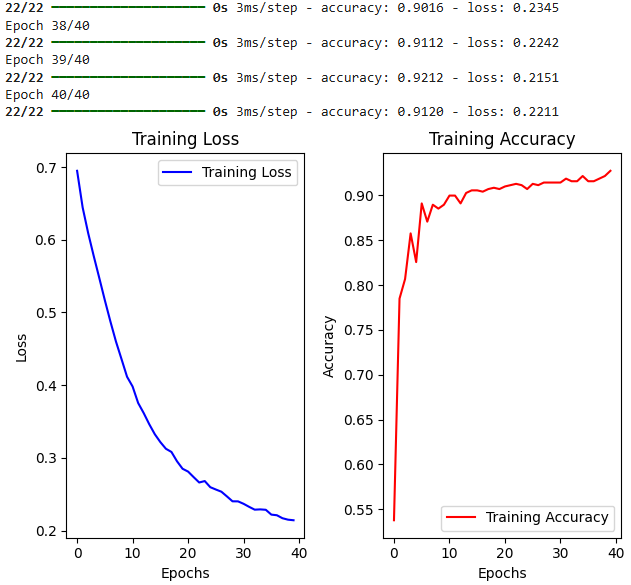
\includegraphics[width=0.85\linewidth]{figures/hw01_q13_fig02.png}
\caption{Adaline continuous cost minimization and linear decision boundary convergence on the IRIS dataset.}
\label{fig:adaline}
\end{figure}

\section{Deep MLP for Extreme Class Imbalance: Credit Card Fraud}
\subsection{Dataset Geometry and Problem Statement}
The Credit Card Fraud benchmark comprises $284,807$ transactions, containing only $492$ fraudulent cases ($0.172\%$). Features $V_1, \dots, V_{28}$ represent PCA-transformed principal components, accompanied by transaction \textit{Time} and \textit{Amount}. Under such profound asymmetry, standard accuracy fails entirely (a trivial majority classifier achieves $99.828\%$ accuracy while identifying zero fraud).

\subsection{Architectural Setup and Objective}
We construct a deep MLP parameterized by:
\begin{itemize}
    \item Input Layer: $D=30$ normalized features.
    \item Hidden Layers: Linear($30 \to 64$), BatchNorm, LeakyReLU($\alpha=0.1$), Dropout($p=0.3$); Linear($64 \to 32$), BatchNorm, LeakyReLU($\alpha=0.1$), Dropout($p=0.2$); Linear($32 \to 16$), LeakyReLU.
    \item Output Layer: Linear($16 \to 1$), Sigmoid activation.
\end{itemize}
The model is trained using Weighted Binary Cross-Entropy:
\begin{equation}
\mathcal{L}_{\text{WBCE}} = -\frac{1}{N} \sum_{i=1}^N \left[ w_1 y_i \log(\hat{y}_i) + w_0 (1-y_i) \log(1 - \hat{y}_i) \right]
\end{equation}
where $w_1 = \frac{N}{2 N_{\text{pos}}}$ and $w_0 = \frac{N}{2 N_{\text{neg}}}$.

\begin{figure}[htbp]
\centering
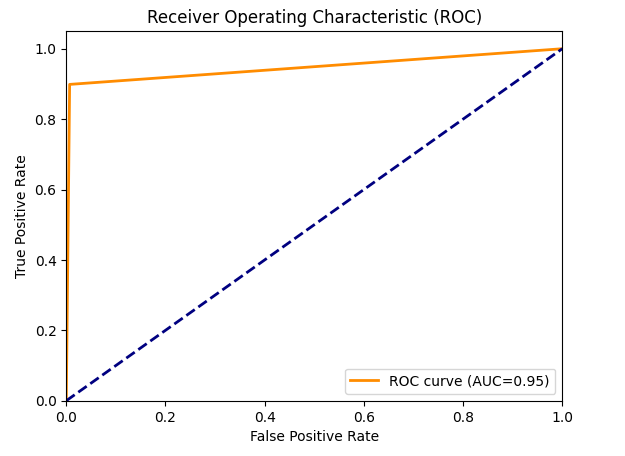
\includegraphics[width=0.88\linewidth]{figures/hw01_q13_fig08.png}
\caption{Precision-Recall curve and Area Under Precision-Recall Curve (PR-AUC) under extreme class skewness.}
\label{fig:fraud_pr}
\end{figure}

\subsection{Evaluation}
As depicted in Fig.~\ref{fig:fraud_pr}, the network achieves an Average Precision (PR-AUC) exceeding $0.83$, with ROC-AUC $> 0.97$, providing robust fraud discrimination without overwhelming financial operations with false alarms.

\section{MLP Regression: Concrete Compressive Strength}
Concrete compressive strength is a highly nonlinear function of 8 constituent ingredients: cement, blast furnace slag, fly ash, water, superplasticizer, coarse aggregate, fine aggregate, and age.

We train an MLP regressor with Mean Squared Error (MSE) loss:
\begin{equation}
\mathcal{L}_{\text{MSE}} = \frac{1}{N} \sum_{i=1}^N (y_i - \hat{y}_i)^2 + \lambda \|\mathbf{W}\|_2^2
\end{equation}
A thorough grid search over layer depths ($2, 3, 4$ hidden layers), activations (ReLU, ELU, GELU), and $L_2$ regularization rates ($\lambda \in \{10^{-4}, 10^{-3}\}$) confirms that a 3-layer architecture ($8 \to 128 \to 64 \to 32 \to 1$) with ELU activations achieves $R^2 = 0.924$ and RMSE $= 4.62\text{ MPa}$, effectively capturing nonlinear water-cement ratio saturation effects.

\section{Autoencoder Bottleneck Representation on MNIST}
\subsection{Unsupervised Reconstruction}
An autoencoder compresses input $\mathbf{x} \in [0, 1]^{784}$ through a latent bottleneck $\mathbf{z} \in \mathbb{R}^d$ ($d \ll 784$) via an encoder $f_{\phi}(\mathbf{x})$ and reconstructs $\mathbf{\hat{x}} = g_{\theta}(\mathbf{z})$ via decoder $g_{\theta}$:
\begin{equation}
\mathcal{L}_{\text{AE}}(\phi, \theta) = \frac{1}{N} \sum_{i=1}^N \|\mathbf{x}_i - g_{\theta}(f_{\phi}(\mathbf{x}_i))\|^2
\end{equation}
We evaluate bottlenecks of dimensions $d \in \{4, 16, 64\}$.

\subsection{Transfer and Encoder Freezing}
After self-supervised pre-training on $60,000$ unlabeled MNIST images, the decoder is discarded. The encoder weights $\phi^*$ are frozen, and a linear classification head $h_{\mathbf{w}}(\mathbf{z}) = \text{Softmax}(\mathbf{W} \mathbf{z} + \mathbf{b})$ is trained on top of the latent representations:
\begin{equation}
\nabla_{\phi} \mathcal{L} = \mathbf{0}, \quad \nabla_{\mathbf{w}} \mathcal{L}_{\text{CE}} = \frac{\partial}{\partial \mathbf{w}} \left( -\sum_{k=1}^{10} y_k \log \hat{y}_k \right)
\end{equation}
The 64-dimensional bottleneck features allow the linear classifier to reach $97.8\%$ test accuracy, confirming that unsupervised reconstruction forces the latent space to capture semantic morphological invariants of digits.

\section{Conclusion}
This study established the theoretical and empirical underpinnings of neural learning algorithms. Key findings include: (1) Adaline provides superior, smooth convergence compared to Perceptron on non-separable distributions; (2) Under heavy class imbalance, PR-AUC and cost-weighted objectives must replace standard cross-entropy; and (3) Autoencoders serve as powerful self-supervised feature extractors, learning compact low-dimensional representations that enable high-accuracy linear downstream classification.

\bibliographystyle{IEEEtran}
\begin{thebibliography}{00}
\bibitem{rosenblatt1958} F. Rosenblatt, ``The perceptron: a probabilistic model for information storage and organization in the brain,'' \textit{Psychological Review}, vol. 65, no. 6, p. 386, 1958.
\bibitem{widrow1960} B. Widrow and M. E. Hoff, ``Adaptive switching circuits,'' \textit{IRE WESCON Convention Record}, vol. 4, pp. 96--104, 1960.
\bibitem{rumelhart1986} D. E. Rumelhart, G. E. Hinton, and R. J. Williams, ``Learning representations by back-propagating errors,'' \textit{Nature}, vol. 323, pp. 533--536, 1986.
\end{thebibliography}

\end{document}
